\chapter[Cellular blebs]{Cell surface mechanochemistry and the determinants of bleb formation, healing and travel velocity}

K. Manakova$^\dag$, H.Yan$^\dag$, J. Lowengrub$^\dag$ and J. Allard$^{\dag\ddag\ast}$\\
$^\dag$Department of Mathematics, Center for Complex Biological Systems, $^\ddag$Department of Physics and Astronomy, University of California, Irvine, $^\ast$Corresponding author \\ 

\section*{Abstract}
%%%%%%%%%%%%%%%%%%%%%%%%%%%%%%%%%%%%%%%%%%%%%%%%%%%

Blebs are pressure driven cell protrusions implicated in cellular functions such as cell division, apoptosis, and cell motility including motility of protease inhibited cancer cells. Because of their mechanical nature, blebs inform us about general cell surface mechanics including membrane dynamics, pressure propagation throughout the cytoplasm, and the architecture and dynamics of the actin cortex. Mathematical models including detailed fluid dynamics have previously been used to understand bleb expansion. Here we develop mathematical models on longer timescales that recapitulate the full bleb life cycle, including both expansion and healing by cortex reformation in 2D and 3D, in terms of experimentally accessible biophysical parameters such as myosin contractility, osmotic pressure, and turnover of actin and ezrin. The model provides conditions under which blebbing occurs, and naturally gives rise to traveling blebs. The model predicts conditions under which blebs travel or remain stationary, and predict the bleb traveling velocity, a quantity that has remained elusive in previous models.  As previous studies have used blebs as reporters of membrane tension and pressure dynamics within the cell, we have used our system to investigate various pressure equilibration models and dynamic, non-uniform membrane tension to account for the shape of a traveling bleb. We also find that traveling blebs tend to expand in all directions unless otherwise constrained, suggesting the importance of cell surface heterogeneity. 

%%%%%%%%%%%%%%%%%%%%%%%%%%%%%%%%%%%%%%%%%%%%%%%%%%%
% !TEX root = Project1.tex

%%%%%%%%%%%%%%%%%%%%%%%%%%%%%%%%%%%%%%%%%%%%%%%%%%%
\section*{Introduction}
%%%%%%%%%%%%%%%%%%%%%%%%%%%%%%%%%%%%%%%%%%%%%%%%%%%



% why the cell surface is important
The eukaryotic cell surface is the site of cell-cell communication \cite{Allard:2012gy}, cell-environ\-ment interactions including motility and mechanosensing \cite{Zhu:2013kq}, and cell morphogenesis \cite{Allard:2012if}, among other processes. Many of these processes involve mechanical forces and deformation, making mechanics of the cell surface an increasingly important topic of investigation.

% why the cell surface is complicated
The study of cell surface mechanics is complicated by dynamic interactions among its multiple constituents with distinct material properties. 
%membrane
The plasma membrane is fluid \cite{Rangamani:2013ce} and resists deformation and experiences surface tension on the order of 10-100 pN/nm \cite{Tinevez:2009bh} that is spatially and temporally non-uniform \cite{Peleg:2011fz}. 
% cortex
Below the membrane is a $\sim100\nm$ layer of F-actin with distinct microarchitecture from the cytoplasmic F-actin further into the cell \cite{Clark:2013ef}, termed the cortex. The cortex is anisotropic poro-viscoelastic material \cite{Salbreux:2009fp,Hannezo:2015ba} that generates internal active contractile stresses by association with myosin \cite{Tinevez:2009bh}. 
% adhesions
The membrane and cortex are decorated with a myriad of molecules, some of which interact with both of them, thereby facilitating dynamic adhesion between them \cite{Fritzsche:2014jw}.   
% big questions about cell surface
This complexity obscures fundamental questions such as, how quickly is hydrostatic pressure propagated through the cortex \cite{Strychalski:2013eo,Charras:2009dp,Clark:2014fj}, or surface tension propagated across the membrane \cite{Peleg:2011fz,BenFogelson:2014gx,Rangamani:2013ce}?
% function
These questions have functional consequences since, for example, membrane bending and tension are implicated in endocytosis \cite{Liu:2010hla}, cell polarization \cite{Weiner:2007gd} and motility \cite{BenFogelson:2014gx, Yip:2015cb}, while the cortex is implicated in cell division, initiating filopodia and other cellular protrusion \cite{Leijnse:2015fd},  both facilitating and preventing vesicle export \cite{Wollman:2012kha},  and wound healing \cite{Salbreux:2009fp}. 
 

% blebs
An example cell process that involves all the above components is offered by cellular blebbing, pressure-driven  protrusions that occur in many cell types and conditions \cite{Charras:2008ic,Charras:2008bz,Paluch:2013ea}. An individual bleb begins with an initiation phase whereupon the membrane separates from the cortex, either spontaneously or under experimental triggering such as laser ablation \cite{Clark:2013ef, Charras:2008ic}. Initiation is followed by a rapid ($\sim10\s$) expansion phase which, unlike other cellular protrusion, is not actively driven by cytoskeletal polymerization \cite{Danuser:2012dr}. After expansion, blebs can exhibit a range of dynamic behaviors: Stationary blebs heal in place with a slower timescale ($\sim$minutes). Other classes of bleb that have been experimentally observed travel around the periphery of the cell --- a phenomenon termed circus movement \cite{Fujinami:1975vo,Anonymous:4HHO02bL,Lim:2012fz} --- or repeatedly bleb on top of an existing bleb \cite{Charras:2008ic}. The complete life-cycle is determined by a complex interplay between flow of cytosol into the bleb, contractive forces in the cortex and the formation and maintenance of membrane-cortex adhesions.
% bleb function
Blebs are implicated in non-lamellipodial cell motility \cite{Logue:2015jj,Charras:2008gf}, including in protease-inhibited cancer cells \cite{Friedl:2003if}; in maintaining homeostasis during division \cite{Sedzinski:2011ef}; and have a speculated role in the origin of eukaryotic life \cite{Baum:2014ee}.

% bleb travel
Traveling waves of protrusion are increasingly reported in different cell types \cite{Weiner:2007gd,Ryan:2012ej}, but these protrusions are typically F-actin-enriched (although see \cite{Kapustina:2013gc}), whereas blebs represent regions with reduced F-actin.
A fundamental question to the understanding of any traveling wave phenomenon \cite{Allard:2012if} is: what determines the traveling velocity of a traveling bleb? And, in the case of blebs which may be stationary or travel, even simultaneously at different locations on the same cell, what determines whether a bleb will travel or heal in place? 

% previous models of blebbing
Several theoretical models of blebbing have been developed to capture various aspects of the process. 
% bob, wanda, Mitran
Computational fluid dynamics models \cite{Strychalski:2013eo,Strychalski:2015fu,Young:2010dp} have been developed to understand the initial expansion phase during which cytosolic fluid follows the protruding membrane. Due to the computational cost of solving the fluid equations along with their mechanical interaction with immersed structures (which typically have sub-second dynamics \cite{Strychalski:2013eo,Strychalski:2015fu}), simulations of these models are typically limited to 2D approximation and seconds timescales. 
% maha
Other researchers \cite{Lim:2012fz} have used force-balance models \cite{Alert:2015gz,Kapustina:2013gc} to obtain computationally tractable models describing the full life cycle. These models are in 2D and must assume an {\it a priori} bleb healing velocity to generate traveling blebs. 
% Baker-Goriely
Continuum analytical models  \cite{Woolley:2013bx,Woolley:2014jm, Woolley:2015jn} have also been developed that move beyond the typical small-deformation approximations typically used to describe membrane geometry. These models capture details of the shape of stationary bleb that have, among other findings, implicated lipid flow in determining bleb behavior. 

% here we
A full, 3D description of the full life-cycle of traveling blebs is therefore lacking. In this work, we develop a model of local cell surface mechanics on timescales of seconds to minutes, thereby including cortex turnover and bleb healing. We exploit two simplifying assumptions: First, we assume hydrodynamic equilibrium is reached rapidly and therefore avoid computationally taxing fluid dynamic simulation, at the expense of losing information about the expansion phase. Second, our model contains a single, ``effective" cortex corresponding to the weighted average of cortical actin, allowing us to include implicitly the cytoskeleton further inside the cell. 

An emerging feature of this model is that transient detachment between membrane and cortex can lead to: 1) rapid healing, 2) stationary bleb formation, and 3) spontaneous bleb travel, depending on model parameters. Our model makes two main contributions: First, since traveling blebs arise naturally, we can  elucidate the determinants of bleb travel. In particular,  
% simplifying assumptions/limitations
several simplifying assumptions allow us to obtain an analytic expression for bleb travel velocity that provides experimentally-accessible perturbations predicted to accelerate or decelerate travel. 
Our second finding is that the biophysical ingredients hypothesized to account for blebbing produce traveling blebs with unrealistic geometry. 
% key insights
This suggests yet-to-be-identified mechanism playing a role in cell integrity and the localization of morphological perturbations. 
We explore the influence of dynamic, non-uniform membrane tension;  hydrostatic pressure equilibration occurring at multiple length scales (i.e., global versus local \cite{Strychalski:2015fu}); and spatial heterogeneity. We find the latter sufficient to maintain bleb compactness during travel.


%%%%%%%%%%%%%%%%%%%%%%%%%%%%%%%%%%%%%%%%%%%%%%%%%%%

%%%%%%%%%%%%%%%%%%%%%%%%%%%%%%%%%%%%%%%%%%%%%%%%%%%
% !TEX root = Project1.tex


%%%%%%%%%%%%%%%%%%%%%%%%%%%%%%%%%%%%%%%%%%%%%%%%%%%
\section{Model}
%%%%%%%%%%%%%%%%%%%%%%%%%%%%%%%%%%%%%%%%%%%%%%%%%%%


Our minimal model, summarized schematically in Fig.~\ref{fig::schematic}, consists of four fundamental dynamic variables, as functions of time $t$ and location on the two-dimensional cell surface, parametrized by $(x_1, x_2)$. The actin cortex, has local height described by $y_C(x_1,x_2,t)$ measured normal to the mean cell surface from its steady-state configuration $y_C=0$, and thickness $c(x_1,x_2,t)$. The cortical-cytoplasmic actin cytoskeleton can in principle have complicated morphologies that cannot be accounted for by a single location $y_C$, so we think of $y_C$ as the weighted average position of maximal cortical actin. Membrane-cortex adhesions are described by density $a(x_1,x_2,t)$ in molecules$/\nm^2$. Finally, the membrane has local height $y_M(x_1,x_2,t)$.  Note that our model is agnostic about the molecular constituents of the membrane, and it could include the plasma membrane as well as permanently membrane-associated proteins and cytoskeletal networks \cite{Kapustina:2013gc}. Our approach is similar to previous descriptions of membrane mechanics \cite{Alert:2015gz,Lim:2012fz,Allard:2012gy,Peleg:2011fz}.

%%%%%%%%%%%%%%%%%%%%%%%%%%%%%%%%%%%%%%%%%%%%%%%%%%%%%%%%%%%%%%%%%%%%%%%%
\begin{figure}
   \begin{center}
   \captionsetup{width=8.5cm}
	\includegraphics*[width=8.5cm]{Project1/figs/figure1.pdf}
      \caption{(A) Micrograph of a single bleb, induced by laser ablation on the surface of a HeLa cell, 43 seconds after initial formation. Taken from \cite{Biro:2013bk}. (B) Model components. At each location on the surface of the cell $x$, four quantities are represented: The height of the membrane $y_M(x,t)$, the height and thickness of the actin cortex $y_C(x,t)$ and $C(x,t)$ respectively, and the local density of membrane-cortex anchoring proteins, $A(x,t)$. Note that the schematic shows the range of possible model states (e.g., thick or thin cortex, protruding or proximal membrane), while specific predicted dynamics will be determined by simulation.}
      \label{fig::schematic}
   \end{center}
\end{figure}
%%%%%%%%%%%%%%%%%%%%%%%%%%%%%%%%%%%%%%%%%%%%%%%%%%%%%%%%%%%%%%%%%%%%%%%%

\paragraph{Assembly and turnover.}
%Cortex
The cortex is an active, anisotropic poro-viscoelastic material \cite{Salbreux:2009fp,Hannezo:2015ba}. Since the molecular details of cortex assembly are still under investigation \cite{Bovellan:2014ka}, we assume simple first-order kinetics,
\begin{align}
\frac{\partial c}{\partial t} &= \omega a - r c. \label{eq::cortexKinetics}
\end{align}
The first parameter $\omega$ governs cortex assembly, and assumes new cortex requires adhesion to a nearby membrane (although existing cortex can exist anywhere), consistent with the observation that cortical actin has different architecture than cytoplasmic F-actin \cite{Clark:2013ef}. The second term describes cortex turnover with rate $r \sim 0.05 \s^{-1}$ \cite{Fritzsche:2014jw}. While we use the term thickness, we interpret $c$ as a combination of density and spatial thickness, with fluorescence intensity of labelled F-actin serving as its experimental proxy. Therefore $c$ has arbitrary units.

%Adhesions
In stereotypical, pre-bleb conditions, the cortex is attached to the membrane via membrane-cortex adhesion molecules including ezrin- radixin- moesin (ERM) family proteins \cite{Fritzsche:2014jw}, as well as any other membrane proteins that interact with F-actin \cite{Paszek:2015it}, therefore we use the generic term ``adhesion" to describe their combined effect. We use similar first-order kinetics for adhesion assembly and turnover, with three additional assumptions: 1) Adhesion assembly saturates at high cortex thickness; 2) Adhesion attachment requires proximity between cortex and membrane, with characteristic distance $\delta$ that describes the ``reach" of adhesion molecules, which may be as large as $\sim100\nm$ \cite{Clark:2013ef}; and 3) Adhesion detachment is force-dependent with characteristic breaking force $f_0$. These assumptions lead to
\begin{align}
\frac{\partial a}{\partial t} &=  \frac{\kon\,c}{c_0+c}\; \mbox{exp}\left( - \left(\frac{y_M-y_C}{\delta}\right)\right) - \koff\, a\; \mbox{exp}\left( \frac{\kappa (y_M-y_C)}{f_0}\right) \label{eq::adhesionKinetics}
\end{align}
where $\kon$ and $\koff$ have units of $\nm^{-2} \s^{-1}$ and $\s^{-1}$, respectively, and $c_0$ is the cortex thickness at which adhesion assembly is half-maximal. The numerator $\kappa (y_M-y_C)$ follows from the assumption that adhesions collectively behave like springs with Hookean stiffness $\kappa$. Note that adhesion turnover $\koff\sim 2\s^{-1}$ \cite{Fritzsche:2014jw} is significantly faster than cortex turnover, leading to a separation of timescales we exploit.

\paragraph{Mechanics.}
The above equations describing assembly and disassembly kinetics are coupled to a mechanical description of the membrane and cortex via mechanical energy,
\begin{align}
E = \iint&\;   \mathcal{H}_1 + \mathcal{H}_M + \mathcal{H}_C \; dx_1 dx_2 \label{eq::energy}
\end{align}
where 
\begin{align}
\mathcal{H}_1 &= \frac{1}{2}a\kappa \left(y_M-y_C\right)^2 - \Pi.
\end{align}
The first term corresponds to tension on the adhesions. Since these adhesions break at moderate tension, we model these as linear springs. The second term is hydrostatic pressure $\Pi$, specified below. Membrane mechanics are described by
\begin{align}
\mathcal{H}_M &= \frac{1}{2}\; \gamma_M \left( \nabla y_M \right)^2 + \frac{1}{2}B_M \left( \nabla^2 y_M \right)^2 
\end{align}
corresponding to the standard Canham-Helfrich energy with membrane tension $\gamma_M$ and bending rigidity $B_M$ \cite{Helfrich:1973td,Alert:2015gz,Woolley:2014jm,Lim:2012fz}. These functional forms represent a small-deformation approximation and comprise a simplifying assumption to make the model more easily amenable to the analysis. We therefore do not expect our model to capture the shape of a fully-expanded bleb with high accuracy, for which geometrically more complex models have been developed \cite{Woolley:2015jn}. Finally, mechanics of the actin-myosin cytoskeleton is included in
\begin{align}
\mathcal{H}_C &= c\sigma_m \left( y_C^2 + \frac{1}{2}\; w_C \left( \nabla y_C \right)^2 \right), 
\end{align}
accounting for active of the cortex, which generates contraction stress $\sigma_m c$, assumed proportional to cortex thickness. The first term accounts for inward contractility, as the cortical cytoskeleton pulls against the cytoplasmic cytoskeleton, generating a normal (inwards) force, {as shown in  Fig. ~\ref{fig::blebgeometry}}. Note this term has been neglected in previous work \cite{Lim:2012fz}. The second term accounts for tangential stress in the plane of the cortex, where $w_C$ is the cortex dimension that translates the 3D contractile stress to a tangential planar contractile tension. Importantly, we find that in traveling blebs, where the cortex is discontinuous, the tangential term does not generate sufficient inward force to heal the tail of the bleb as it travels, highlighting the importance of the normal contractility term. Cortex elasticity terms describing how the cortex resists deformation are straightforward to add, however we find that their omission is sufficient to explain our key results. 

The mechanical features included in the energy Eq.~\ref{eq::energy} can also be understood by their equivalent force-balance form, Eq.~\ref{eq::forceBalanceCortex}-\ref{eq::forceBalanceMembrane} below.




% pressure
Pressure propagation inside the complex rheology of the cytoplasm is under intense investigation \cite{Charras:2005dm, Strychalski:2013eo, Sedzinski:2011ef}. To address the nature of pressure dynamics, we investigate several pressure model variants. As a base model, we assume pressure is locally relaxed when the membrane is allowed to relax, 
\begin{equation}
\Pi = \hat{\Pi}\cdot \left(1 - \frac{y_M}{2 y_M^0} \right)^2 \label{eq::localPressure}
\end{equation}
where $y_M^0$ sets the characteristic distance at which pressure is significantly reduced. The pressure drop would be lessened if the membrane is locally water-permeable \cite{Taloni:2015}, which would have the effect of reducing the coefficient relating pressure to membrane extrusion. Other model variants explore the possibility of rapidly-equilibrated pressure across the whole cell surface and a mixture of global and local pressure relaxation.  

% membrane tension
The dynamics of membrane tension are also under investigation \cite{BenFogelson:2014gx,Peukes:2014fw,Tinevez:2009bh,Weiner:2007gd,Allard:2012if}. Under the simplest assumption, membrane tension $\gamma_M$ is spatially uniform and constant in time. We use this as our base model, but also explore membrane tension that is spatially non-uniform and dynamically responding to local stretching/unruffling and cortex attachment in Results. 

\paragraph{Preliminary analysis.}
Taking the variational derivative of Eq.~\ref{eq::energy} leads to force-balance equations on the cortex and membrane,
\begin{align}
0 &= + a \kappa (y_M-y_C) - \sigma_m c y_C + \sigma_m c\, w_C \nabla^2  y_C \label{eq::forceBalanceCortex}\\
0 &= - a\kappa (y_M-y_C) + \frac{\delta \hat{\Pi}}{\delta y_M}  + \gamma_M \nabla^2  y_M - \beta\;\nabla^4 y_M \label{eq::forceBalanceMembrane}
\end{align}
Physical parameters are summarized in Table~\ref{tab:modelparameters}. 
%%%%%%%%%%%%%%%%%%%%%%%%%%%%%%%%%%%%%%%%%%%%%%%%%%%%%%%%%%%%%%%%
\begin{table}[t!]
\caption{Model parameters.}\centering \label{tab:modelparameters} 
\begin{tabular}{ c  l  l}
\hline
Symbol & Dimensions & Meaning \\
\hline
$\omega$ & [A.U.] $\cdot \s^{-1}$ & Cortex assembly rate constant  \\
$r$ & $\s^{-1} $ & Cortex turnover rate constant \\
$\kon$ & $\nm^{-2}\s^{-1}$ & Adhesion assembly rate  \\
$\koff $& $ \s^{-1}$ & Adhesion turnover rate \\
$c_0$ & [A.U.] & Cortex thickness at adhesion saturation \\
$\delta$ &  $\nm$& Adhesion length between cortex and membrane \\
$\kappa$ & $\pN/\nm$ & Adhesion spring constant \\
$f_0$ & $\pN$ &Adhesion breaking strength\\
$\gamma_M$ & $ \pN/\nm$ & Membrane tension \\
$B_M$& $\pN\nm$ & Membrane bending modulus \\
$\sigma_m$ & $ \mbox{Pa}$ / [A.U.] & Actin-myosin contractility (per unit of $c$) \\
$\hat\Pi$ & $ \mbox{Pa}$/nm & Hydrostatic pressure scale \\
\hline
\end{tabular}
\end{table}
%%%%%%%%%%%%%%%%%%%%%%%%%%%%%%%%%%%%%%%%%%%%%%%%%%%%%%%%%%%%%%%%
Values for many of these parameters have been estimated, see Fig. ~\ref{fig::blebgeometry}. The spatial terms significantly complicate both numerical solution and analysis of the model, and we find that their omission does not significantly influence blebbing dynamics. This is expected for membrane bending, since bending forces are expected to be negligible on length scales above $\sim (\beta/\gamma_M)^{(1/4)}\sim100\nm$ \cite{Allard:2012gy}. Therefore, unless otherwise noted below, we neglect the tangential cortex stress $\nabla^2y_C$ and membrane bending $\nabla^4 y_M$ terms. However, see Appendix ~\ref{sec:project1} for solutions with full terms. 

We non-dimensionalize by choosing a characteristic actin cortex thickness, $C_c= c_0$, a characteristic density of adhesions, $A_c =  \kon/\koff$, a characteristic time, $t_c=1/r \sim 30\s$ \cite{Fritzsche:2014jw}, and a characteristic position, $Y_c=y_M^0$, and a characteristic length by $x_c =\sqrt{2 \gamma_M \koff/(\kon \kappa)} \sim 0.2\mum$, resulting in a non-dimensional model, 
\begin{align}
\dfrac{dC}{d \tau}  & =  \Omega A - C\label{eq::nondimC}\\
\epsilon\dfrac{dA}{ d \tau}  & =  \dfrac{C}{1+C} \mbox{exp}\left(-\dfrac{Y_M-Y_C}{D}\right) - A \mbox{exp} \left(\dfrac{Y_M-Y_C}{F_0} \right) \label{eq::nondimA}\\
0 & = A(Y_M-Y_C) - MCY_C \label{eq::nondimyM}\\
0 & = -A(Y_M-Y_C) + P(1-Y_M) +  \frac{\partial^2 Y_M}{\partial \chi^2} \label{eq::nondimyC}
\end{align}
with six nondimensional parameters defined in Table~2. 

Here we provide an overview of the roles of each term in Eq.~\ref{eq::nondimC}-\ref{eq::nondimyC}. The first and second term in the $C$ equation describe cortex formation and turnover, respectively. The first and second term in the $A$ equation describe attachment and detachment of cortex-membrane adhesions. The first exponential in Eq.~\ref{eq::nondimA} arises because the membrane and cortex must be in proximity for an adhesion to form. The second exponential in Eq.~\ref{eq::nondimA} describes the accelerated breaking of adhesions under force. Then, Eqs.~\ref{eq::nondimyM} and~\ref{eq::nondimyC} describe the mechanical balance between five forces acting on the membrane and cortex. The forces, in order of appearance, are: Adhesion force on the cortex; myosin contractility of the cortex; adhesion force on the membrane; pressure; and membrane tension.

Note that our choice of nondimensionalization means that only relative changes in $Y_M$ and $Y_C$ are physically meaningful. We numerically solve these equations as described in Appendix ~\ref{sec:project1}. \cite{wise07}. 




%%%%%%%%%%%%%%%%%%%%%%%%%%%%%%%%%%%%%%%%%%%%%%%%%%%%%%%%%%%%%%%%
\begin{table}[t!]
\caption{Non-dimensional parameters.}\centering \label{tab:par} 
\begin{tabular}{ c  l  l}
\hline
Symbol & Definition & Interpretation \\
\hline
$ \Omega$ &  ${ \omega  \kon} / {\gamma c_0 \koff}$ & Cortex intensity\\
 $\epsilon$ &  ${ r} / {\koff}$& Ratio of adhesion and cortex turnover times\\
$D$ &  ${ \delta} / {y_M^0}$&Adhesion reach \\
$F_0$ &  ${ f_0} / {\kappa y_M^0}$&Adhesion bond strength\\
$M$ &  ${\sigma_m c_0 \koff} / {\kon \kappa}$ &Myosin contractility relative to adhesion strength\\
$P$ &  ${\hat{\Pi} \koff} / {\kon \kappa}$ & Pressure relative to adhesion strength\\
\hline
\end{tabular}
\end{table}
%%%%%%%%%%%%%%%%%%%%%%%%%%%%%%%%%%%%%%%%%%%%%%%%%%%%%%%%%%%%%%%%



%%%%%%%%%%%%%%%%%%%%%%%%%%%%%%%%%%%%%%%%%%%%%%%%%%%

%%%%%%%%%%%%%%%%%%%%%%%%%%%%%%%%%%%%%%%%%%%%%%%%%%%
% !TEX root = bleb.tex


%%%%%%%%%%%%%%%%%%%%%%%%%%%%%%%%%%%%%%%%%%%%%%%%%%%
\section*{Results}
%%%%%%%%%%%%%%%%%%%%%%%%%%%%%%%%%%%%%%%%%%%%%%%%%%%


%%%%%%%%%%%%%%%%%%%%%%%%%%%%%%%%%%%%%%%%%%%%%%%%%%%
\paragraph{Model exhibits  blebbing and non-blebbing behaviors.}
%%%%%%%%%%%%%%%%%%%%%%%%%%%%%%%%%%%%%%%%%%%%%%%%%%%
The quantitative model combines five mechanisms of the membrane-cortex interaction: force-sensitive adhesions, local hydrostatic pressure, cortex contractility, membrane tension and cortex turnover. We numerically simulate the model and find three classes of dynamics arise from the same model at different parameters: Stable non-blebbing states, stationary blebbing, and traveling blebs. We discuss these in turn.

% stationary blebs
At equilibrium, the membrane and cortex are locally approximately flat. We apply an initial perturbation corresponding to local ablation by locally reducing the adhesion density by 99\%. In blebbing states, the membrane will detach from the cortex and protrude locally. The membrane  then continues to move away from the thinning cortex as the detached region grows in both lateral size (along the surface) and in height (i.e., normal to the cell surface) until it reaches a maximum size around $\tau=1.75$. The adhesions subsequently accumulate under the protruding membrane and the cortex is able to re-attach and thicken. Under the influence of cortex contraction, the bleb heals and the membrane returns to its equilibrium. This bleb-like behavior is observed in 2D (Fig.~\ref{fig::stationary}A left) and in 3D (Fig.~\ref{fig::stationary}B) simulations. 
% stable
In contrast, at different biophysical parameters, the detached region of membrane may not grow after perturbation, but instead directly and rapidly return to equilibrium, shown in Fig.~\ref{fig::stationary}A right. This stable behavior is observed in both 2D (Fig.~\ref{fig::stationary}A right) and in 3D (not shown). 

%%%%%%%%%%%%%%%%%%%%%%%%%%%%%%%%%%%%%%%%%%%%%%%%%%%%%%%%%%%%%%%%%%%%%%%%
\begin{figure}
\captionsetup{width=17cm}
	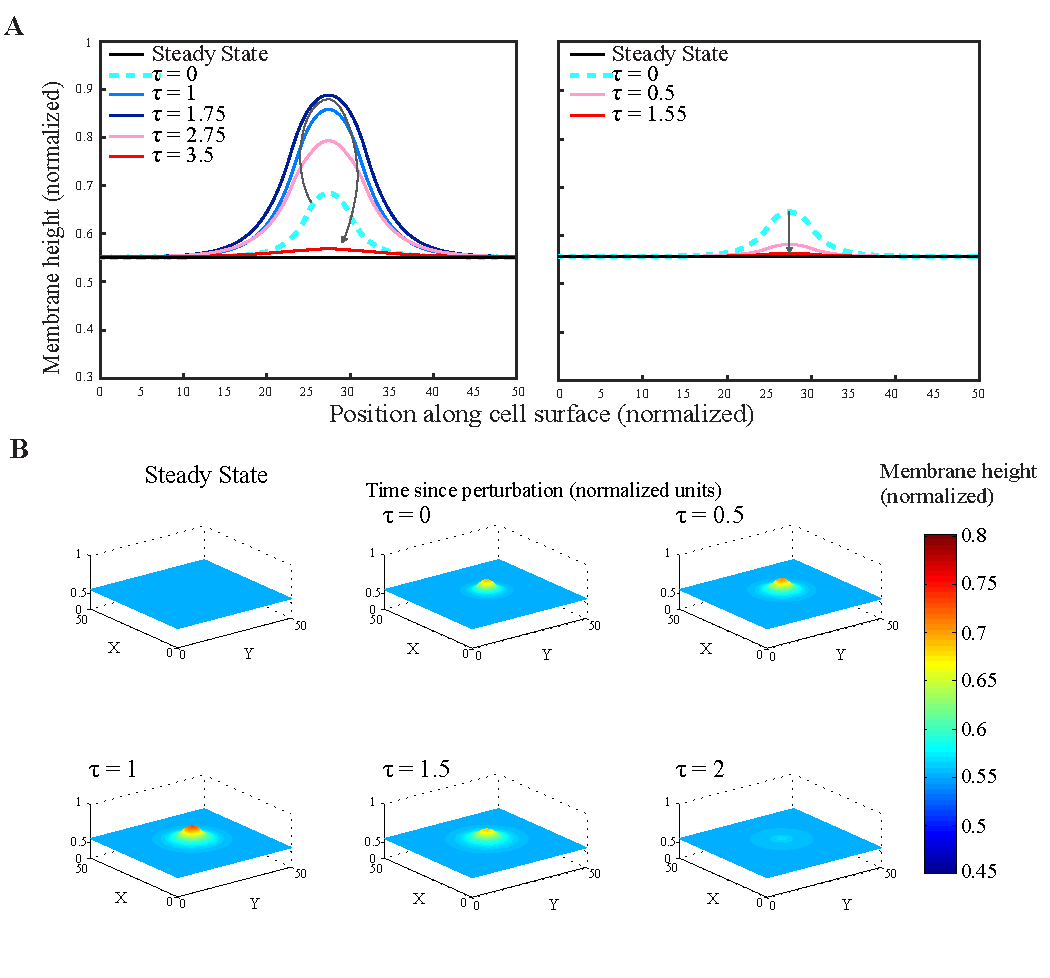
\includegraphics[width=17cm,center]{Project1/figs/figure2}
      \caption{Model exhibits stationary blebs and non-blebbing states in 2D and 3D. (A) Profile of stationary solution of the 2D system: (Left) Excitable state in which an initial perturbation (cyan dashed) expands in both height (normal to cell surface) and laterally along cell surface before retracting. (Right) Non-excitable state in which the initial perturbation rapidly and directly returns to equilibrium. Parameter values: $\Omega = 40$, $\epsilon = 0.1$, $F_0 = 1$, $M = 0.007$, $P = 0.1$ and $D = 0.15$ for the excitable state, $D = 0.2$ for the non-excitable state. (B) Profile of stationary solution  of the 3D system in an excitable state. Parameter values: $\Omega = 50$, $\epsilon = 0.1$, $F_0 = 1$, $M = 0.007$, $P = 0.1$ and $D = 0.15$. Note that our choice of nondimensionalization means that only relative changes in $Y_M$ and $Y_C$ are physically meaningful.}
      \label{fig::stationary}
\end{figure}
%%%%%%%%%%%%%%%%%%%%%%%%%%%%%%%%%%%%%%%%%%%%%%%%%%%%%%%%%%%%%%%%%%%%%%%%


%Interestingly, the model can also exhibit another bleb-like behavior. In this third scenario, the membrane will continue to move away from the thinning cortex and grow in size and manages to trigger a travelling wave of membrane detachment followed by a travelling wave of cortex contraction. This travelling bleb behavior is observed in 2D (Figure 4A) and in 3D (Figure 4B).



%%%%%%%%%%%%%%%%%%%%%%%%%%%%%%%%%%%%%%%%%%%%%%%%%%%
\paragraph{Blebs as excitable phenomena}
%%%%%%%%%%%%%%%%%%%%%%%%%%%%%%%%%%%%%%%%%%%%%%%%%%%

% simplification to ODEsys
While numerical simulation of the full model reveals a range of blebbing behavior, we seek to elucidate how biophysical parameters determine the class of dynamics, specifically whether or not a bleb forms. To this end, we simplify the model by neglecting the tension term in Eq.~\ref{eq::nondimyM}. Heuristically, we model an (unrealistic) system in which a patch of cell surface has been cut off from its neighbors (as in Fig. \ref{fig::blebgeometry}). This transforms the force-balance equations Eq.~\ref{eq::nondimyM}-\ref{eq::nondimyC} into a pair of algebraic equations,
\begin{align}
Y_M &= \frac{(A+CM)P}{A MC + AP + MCP}\label{eq::ODEyM}\\
Y_C &= \frac{AP}{A MC + AP + MCP}\label{eq::ODEyC},
\end{align}
shown in Fig.~\ref{fig::ODE}A as a function of $A$ and $C$. These are then substituted into the assembly/disassembly equations, yielding
\begin{align}
\frac{d C}{d \tau} &= \Omega A - C \label{eq::ODEC}\\
\epsilon \frac{d A}{d \tau} &= \frac{C}{1+C} \mbox{exp}\left( -\frac{1}{D} \frac{MP C}{A MC + AP + MCP}\right) \notag\\
 &- A\; \mbox{exp}\left( + \frac{1}{F_0}\frac{MP C}{A MC + AP + MCP}\right) \label{eq::ODEA}
\end{align}
The model is now a system of two ordinary differential equations (ODEs) amenable to phase plane analysis \cite{Keshet}. We plot nullclines in which $dA/d\tau=0$ (green) or $dC/d\tau=0$ (orange) in Fig.~\ref{fig::ODE}B,D.
% nullcline analysis
Four regimes of behavior are observed in this system: 
% monostable
In one (top-left), there is a single stable equilibrium with no threshold behavior. In this regime, perturbations rapidly return to their steady state. We identify this with the stable non-blebbing behavior of the full model. 

%%%%%%%%%%%%%%%%%%%%%%%%%%%%%%%%%%%%%%%%%%%%%%%%%%%%%%%%%%%%%%%%%%%%%%%%
\begin{figure}
   \begin{center}
   \captionsetup{width=17cm}
     \includegraphics*[width=17cm,center]{Project1/figs/figure3}
      \caption{Emergence of blebbing states can be understood in terms of the local $A-C$ phase plane. (A) Since the model assumed force-balance between adhesions, cortex and membrane, a particular value of $A$ and $C$ determine the current position of the membrane and cortex $y_M$ and $y_C$ via Eq.~\ref{eq::ODEyM}-\ref{eq::ODEyC}. (B) Range of behaviors of the system of equations given different parameter sets visualized by the nullclines (orange for $C$ and green for $A$) of the non-dimensionalized  system of equations, Eq.~\ref{eq::ODEA}-\ref{eq::ODEC}. Sample trajectories are shown in black. Monostable parameters:  $\Omega = 100$, $\epsilon = 0.1$, $F_0 = 6.3$, $M = 0.09$, $P = 0.08$ and $D = 0.23$. Bistable parameters:  $\Omega = 6.5$, $\epsilon = 0.1$, $F_0 = 2.9$, $M = 0.43$, $P = 0.016$ and $D = 0.19$. Oscillatory parameters:  $\Omega = 100$, $\epsilon = 0.1$, $F_0 = 1$, $M = 0.007$, $P = 0.1$ and $D = 0.15$. Excitable parameters:  $\Omega = 10$, $\epsilon = 0.1$, $F_0 = 1$, $M = 0.007$, $P = 0.1$ and $D = 0.15$. (C) Time series plot of membrane position (blue) and cortex thickness (orange) beginning in steady state, with a perturbation at time $\tau = 2.5$. (D) The effect of parameter variation on the nullclines. Parameters which are not being varied as indicted in legend are fixed as: $\Omega = 10$, $\epsilon = 0.1$, $F_0 = 1$, $M = 0.007$, $P = 0.1$ and $D = 0.15$. }
      \label{fig::ODE}
   \end{center}
\end{figure}
%%%%%%%%%%%%%%%%%%%%%%%%%%%%%%%%%%%%%%%%%%%%%%%%%%%%%%%%%%%%%%%%%%%%%%%%


% excitable
The stable equilibrium can exhibit excitability (bottom-left), a threshold phenomenon in which small perturbations rapidly return to the equilibrium, but a large sufficiently large perturbation results in a large, slow excursion in parameter space that eventually returns to the equilibrium. We identify this with blebbing behavior in the full model and is characterized by a fold in the $dA/d\tau$ nullcline. 

% chronological narrative of excitation
One such excitation trajectory is shown in Fig.~\ref{fig::ODE}C. 
% note oscillation, cite Clark
Prior to the initial perturbation, $\tau<2$, the flat surface is stable to small perturbations but susceptible to large perturbations such as the decrease in adhesion density applied here at $\tau=2$. The membrane rapidly finds a new mechanical equilibrium, pushed out by hydrostatic pressure which is no longer in competition with cortical contraction. The comparatively slow timescale of cortical turnover (orange curve) leads to a delay before cortex begins to reform ($\tau\approx 4)$, after which the cortex accumulates, pulling in the membrane. Note that many excitable trajectories exhibit low-amplitude oscillations in the cortex as it heals, corresponding to a slight ``over-shooting" of the equilibrium ($\tau\approx 7$). Interestingly, such overshooting has been observed experimentally \cite{Clark:2013ef}.

% threshold
The minimum threshold to initiate an excitation can be extracted from Fig.~\ref{fig::ODE} as follows: The stable equilibrium is at the intersection of the two nullclines. From this point, removing adhesions corresponds to moving horizontally to the left. When adhesion removal is sufficient to cross the $dA/d\tau$ nullcline, an excitation is initiated. Since the $dA/d\tau$ nullcline determines this threshold, it is independent of membrane tension. This is in disagreement with previous estimates of the threshold, where membrane tension has been predicted to be a strong determinant of the size of initial ablation required for bleb initiation \cite{Charras:2008bz}. In contrast, our model predicts that membrane tension determines how big a bleb grows (laterally), but not whether it initially grows. This tension-independence arises heuristically because, once a patch of membrane has been de-adhered, membrane tension promotes bleb growth by pulling neighboring adhesions, and inhibits bleb growth by pulling in the de-adhered region. By the force-balance condition (Eq.~\ref{eq::forceBalanceMembrane}), these forces are equal.

% bistable, oscillatory
We also observe oscillations (bottom-right), which could represent continually blebbing cells \cite{Charras:2008ic}. At yet other parameters, the same model exhibits bistable states (top-right) in which the flat, unperturbed equilibrium is stable, but is accompanied by a second state in which all adhesions are broken, and hydrostatic pressure is too great for the actin cortex to overcome, thus healing does not spontaneously occur. We expect this permanently-damaged state to not be observed experimentally as other cellular processes adjust to heal the cortex.  

% -- parameter variation
Thus, by observing the nullclines  for different parameters, our model makes predictions about the emergence of blebbing following changes in biophysical parameters (Fig.~\ref{fig::ODE}D). We summarize these predictions here and in {Table \ref{tab:predictions}}. Increasing the effective reach of adhesion molecules corresponds to increasing $D$, and abolishes excitability, while decreasing $D$ is predicted to not abolish blebbing but extends the excitable trajectory, therefore predicting a slower healing period. Increasing hydrostatic pressure, e.g., by decreasing extracellular pressure by modulating osmolites, leads to emergence of blebbing from non-blebbing states, in agreement with experiment \cite{Tinevez:2009bh} and intuition. Decreasing myosin contractility abolished excitability, while increasing it delays healing. 


%%%%%%%%%%%%%%%%%%%%%%%%%%%%%%%%%%%%%%%%%%%%%%%%%%%
\paragraph{Biophysical determinants of travel and travel velocity}
%%%%%%%%%%%%%%%%%%%%%%%%%%%%%%%%%%%%%%%%%%%%%%%%%%%

% traveling blebs in 2D model
The previous section's analysis predicts when the cell surface will be excitable and how the bleb evolves in height, but not its dynamics along the cell surface. To understand bleb travel, we return to the full, spatially-extended model first in 2D, then in~3D. 

Excitable parameter sets all spread laterally. However, some parameter sets expand in a limited manner (Fig.~\ref{fig::stationary}A), which we identify as stationary blebs, while others trigger traveling pulses that persists, as shown in Fig.~\ref{fig::travel}A. We identify these as traveling blebs. In 2D, they move in both directions from the site of initial triggering. The time interval $\tau_{\mbox{\scriptsize heal}}$ from triggering and expansion to healing is equal to the healing time in the local analysis and is determined by the cortex turnover time $\tau_{\mbox{\scriptsize heal}} \sim 1/r$. The width of the traveling bleb $w$ is thus determined by its travel velocity, $w\sim v\tau_{\mbox{\scriptsize heal}}$. 

%%%%%%%%%%%%%%%%%%%%%%%%%%%%%%%%%%%%%%%%%%%%%%%%%%%%%%%%%%%%%%%%%%%%%%%%
\begin{figure}
   \begin{center}
   \captionsetup{width=17cm}
     \includegraphics*[width=17cm,center]{Project1/figs/figure4}
      \caption{Traveling blebs in 2D and 3D. (A) Profile of a traveling blebs in 2D after a perturbation at time $\tau =0$. Membrane height in blue,  cortex thickness in orange. Parameter values: $\Omega = 55$, $\epsilon = 0.1$, $F_0 = 1$, $M = 0.007$, $P = 0.1$ and $D = 0.15$. (B) Profile of a traveling bleb in 3D after a perturbation at time $\tau =0$ in the spatial-heterogeneity hypothesis model as shown in top panel, see Results.}
      \label{fig::travel}
   \end{center}
\end{figure}
%%%%%%%%%%%%%%%%%%%%%%%%%%%%%%%%%%%%%%%%%%%%%%%%%%%%%%%%%%%%%%%%%%%%%%%%

% Maxwell
Traveling pulses are a generic feature of spatially-extended excitable systems \cite{Idema:2013ig, Ryan:2012bq, bement2015activator}. In many cases, neighboring regions are coupled by the diffusion of a molecular participant. In these reaction-diffusion systems, a simple mathematical condition exists for determining whether an excitation will induce a traveling pulse or remain localized, sometimes called the Maxwell condition \cite{Anonymous:OS1MPwCl,Mori:2008hj}. Since our system is not a reaction-diffusion system, the Maxwell condition fails to predict whether the blebs travel or not. 

% Velocity analytical form
A major goal of this work is to elucidate the determinants of the traveling velocity, which is known for reaction-diffusion waves and mechanical linear waves \cite{Allard:2012if}. Parameter variations, shown in Fig.~\ref{fig::velocity}, reveal that the parameter regime that allows traveling blebs is narrow in all non-dimensional parameters except $\epsilon$. Indeed, its relative range is less than $10^{0.3}$, corresponding to a 2-fold change. The model therefore predicts a non-dimensional velocity $V\sim 1/\epsilon$, yielding the following dimensional velocity, the principle result of this work:  
\begin{align}
v &\approx \sqrt{\frac{\gamma_M \koff^3}{\kappa \kon}}\; h(\Omega,D,F_0,P,M)\\
 &\approx \sqrt{\frac{\gamma_M \koff^3}{\kappa \kon}} \label{eq::dimVelocity}
\end{align}
where the function $h$ expresses to a weak dependence. We confirm this prediction in Fig.~\ref{fig::velocity}B by performing a large pan-parametric search through parameter space. 
% Predictions for experimental perturbations 
% in equation, not easily abolished; in figure, easily abolished
Eq.~\ref{eq::dimVelocity} predicts that travel will accelerate with increasing membrane tension, with a specifically square-root dependence, and will decelerate with adhesion formation rate $\kon$, a parameter that could be varied by increasing the abundance of total adhesion molecules. The affinity of adhesions for the cortex, $K_A\equiv \kon/\koff$, is also predicted to have a decelerating influence on bleb travel. Interestingly, all other parameters, including hydrostatic pressure and myosin contractility, are predicted to have only a minor influence on travel velocity. Note, however, that these parameters strongly determine whether or not a bleb can form, and whether or not the bleb travels laterally. This model prediction is distinct from a previous prediction \cite{Lim:2012fz}, which posited that cortex healing has an intrinsic velocity, and that this velocity determines bleb travel velocity.  



%%%%%%%%%%%%%%%%%%%%%%%%%%%%%%%%%%%%%%%%%%%%%%%%%%%%%%%%%%%%%%%%%%%%%%%%
\begin{figure}
   \begin{center}
   \captionsetup{width=17cm}
     \includegraphics*[width=17cm,center]{Project1/figs/figure5}
      \caption{Velocity of traveling blebs. A) Plot of each of the 6 non-dimensional parameters, $\Omega$, $D$, $F_0$, $P$, $M$, $\epsilon$, versus non-dimensional velocity. Parameter ranges show the full extent of the parameter regime exhibiting traveling solutions. Fixed parameters in each plot are: $\Omega = 55$, $\epsilon = 0.1$, $F_0 = 1$, $M = 0.007$, $P = 0.1$ and $D = 0.15$. (B) Plot of hypothesized relationship between velocity, Eq.~\ref{eq::dimVelocity}, versus velocity observed in numerical simulation.}
      \label{fig::velocity}
   \end{center}
\end{figure}
%%%%%%%%%%%%%%%%%%%%%%%%%%%%%%%%%%%%%%%%%%%%%%%%%%%%%%%%%%%%%%%%%%%%%%%%

%%%%%%%%%%%%%%%%%%%%%%%%%%%%%%%%%%%%%%%%%%%%%%%%%%%
\paragraph{Hypotheses for compact traveling blebs}
%%%%%%%%%%%%%%%%%%%%%%%%%%%%%%%%%%%%%%%%%%%%%%%%%%%

% bull's eye, generic feature of excitability in 2D
In 3D, the base model also exhibits excitations that either travel or heal in place, in agreement with the local analysis and 2D model. Parameter conditions for excitability and travel are the same as for the 2D model, as is travel velocity. However, we find that a localized initial perturbation spreads radially in all directions, leading to an expanding bull's-eye or target pattern, Fig.~\ref{fig::variants}B. This is a generic feature of excitable systems and arises because of  inherent symmetry: a protruding region of membrane will pull neighboring regions of membrane, without directional bias. 

Since traveling blebs are not experimentally observed to expand in bull's eye patterns, we are led to investigate the question of what gives rise to spatially compact traveling blebs? That is, what breaks the symmetry, inducing travel in a single direction? 

% three hypotheses
We introduce three hypotheses. The first is that hydrostatic pressure may be reduced globally fast enough that, once the excited region enlarges past a certain size, there is no longer sufficient pressure to drive further excitation, thus limiting the target pattern to a compact region. In our model, we modify the membrane force-balance equation, Eq.~\ref{eq::forceBalanceMembrane}, by including the pressure term
% pressure
\begin{equation}
\Pi = \hat{\Pi}\cdot \iint  \left(1 - \frac{y_M}{2y_M^0}\right)\, dx_1 dx_2 \label{eq::globalPressure}.
\end{equation}
This equation corresponds to a shared, global pressure that responds to pressure release (via membrane protrusion) instantly anywhere in the domain. We variously simulated purely global pressure, purely local pressure, and pressure with both local and global equilibration, following recent theoretical evidence \cite{Strychalski:HizQv1Ti}. 

We find that global pressure dynamics can limit the bleb's outward growth when $\hat{\Pi}$ is sufficiently large. However, we do not see symmetry breaking, even upon introduction of $10\%$ parametric noise (Fig.~\ref{fig::variants}A). Interestingly, at intermediate global pressures, the bleb does not heal and instead undergoes slow oscillations (Fig.~\ref{fig::variants}A right). These oscillations reveal an inherent negative feedback between cortical formation, which builds pressure, which in turn breaks adhesions, weakening the cortex.

% tension
The second hypothesis is that bleb compactness and asymmetry is due to a dynamic, non-uniform membrane tension. Following recent evidence \cite{Peukes:2014fw}, we introduce the assumption that tension increases with increasing local cortical actin contractility,
\begin{equation}
\gamma_M = \gamma_{M0} + \gamma_{M1} C\label{eq::nonuniformTension}. 
\end{equation}
We find that this is sufficient to terminate the protrusion (Fig.~\ref{fig::variants}B), but, again, do not observe symmetry breaking.

%%%%%%%%%%%%%%%%%%%%%%%%%%%%%%%%%%%%%%%%%%%%%%%%%%%%%%%%%%%%%%%%%%%%%%%%
\begin{figure}
   \begin{center}
   \captionsetup{width=17cm}
     \includegraphics*[width=17cm,center]{Project1/figs/figure6}
      \caption{Alternative hypotheses for hydrostatic pressure and membrane tension dynamics. (A) Profile of 3D bleb using the global pressure model, Eq.~\ref{eq::globalPressure}, which assumes pressure equilibrates instantaneously across the domain. The bleb expands and contracts in oscillatory cycles (right panel). (B) Profile  of a 3D bleb using a non-uniform tension model, Eq.~\ref{eq::nonuniformTension}, which assumes membrane tension depends on to the cortex thickness at a given point on the membrane. As the strength of this dependence increases (bottom row), the bleb no longer travels across the membrane. Here, $\Gamma = \gamma/\gamma_0$ is the non-dimensionalized membrane tension.}
      \label{fig::variants}
   \end{center}
\end{figure}
%%%%%%%%%%%%%%%%%%%%%%%%%%%%%%%%%%%%%%%%%%%%%%%%%%%%%%%%%%%%%%%%%%%%%%%%

% heterogeneity
Our third hypothesis is that large-length-scale heterogeneity, specifically on the $\sim$ micron length scale of blebs, exists in the local density of proteins such as adhesion molecules and cortical actin nucleators. These manifest as spatial heterogeneity in model parameters such as $D$ and $\Omega$. Since these parameters sensitively determine whether the bleb can travel, such heterogeneity might create specific paths, forcing traveling blebs from spreading in all directions. We simulate the model on a surface in which a small rectangular region has distinct parameters from its surrounding region, as shown in Fig.~\ref{fig::travel}B top. Since the parameter region allowing traveling blebs is fairly narrow (Fig.~\ref{fig::velocity}), it is straightforward to find parameter sets with less than 2-fold variation for which the equilibrium is the same, but only one allows travel. As expected, blebs initiated in the excitable-travel region remain compact and move with velocity $v$ from Eq.~\ref{eq::dimVelocity}, and front-to-back width $w\sim v\tau_{\mbox{\scriptsize heal}}$. 

We conclude that small differences across large length scales in the underlying biophysical properties of the cell surface are sufficient to explain compact traveling blebs. This hypothesis makes the prediction that subsequent traveling blebs will tend to occur in the same location on the cell surface, provided that the heterogeneity's own timescale of variation is longer than the bleb lifetime. %Interestingly, this is qualitatively observed in, e.g., \cite{blebTravelRepeatsDomain}. 



%%%%%%%%%%%%%%%%%%%%%%%%%%%%%%%%%%%%%%%%%%%%%%%%%%%

%%%%%%%%%%%%%%%%%%%%%%%%%%%%%%%%%%%%%%%%%%%%%%%%%%%
% !TEX root = Project1.tex


%%%%%%%%%%%%%%%%%%%%%%%%%%%%%%%%%%%%%%%%%%%%%%%%%%%
\section*{Discussion}
%%%%%%%%%%%%%%%%%%%%%%%%%%%%%%%%%%%%%%%%%%%%%%%%%%%



%Excitability as recurrent theme in Cell Bio
Excitability is a recurrent theme in cell biology \cite{Huang:2013ge,Xiong:2010fb,FitzHugh:1961il, bement2015activator}. We find that the conditions for excitability emerge naturally from the mechanical properties of the cell surface, namely: the combination of a contractile cortex, a membrane exposed to internal hydrostatic pressure, and force-sensitive adhesions connecting them. In addition, membrane mechanical properties (i.e. surface tension) are sufficient for this excitability to lead to either limited-growth stationary blebs that heal in place, or traveling blebs reminiscent of circus movement. Notably, three classes of dynamics arise from the same model at different parameters: Stable, non-blebbing states (Fig.~\ref{fig::stationary}B), stationary blebbing (Fig.~\ref{fig::stationary}A,C); and traveling blebs (Fig.~\ref{fig::travel}A,B). Thus our model provides quantitative conditions for bleb growth and whether the bleb heals locally or travels. 

The model makes two main contributions. First, it allows elucidation of the determinants of the travel velocity in terms of biophysical parameters such as membrane tension and adhesion kinetics, Eq.~\ref{eq::dimVelocity}. Surprisingly, we find that hydrostatic pressure and myosin contractility only weakly determine velocity, while strongly determining other features such as whether the bleb forms, and its height. This is in distinction to previous assumptions \cite{Lim:2012fz} and other traveling waves in biology \cite{Allard:2012if}. 

%Why don't blebs spread as target patterns? Graded Radial Extension, membrane tension must spatially vary
Our second finding is that known biophysical mechanisms are insufficient to account for the compactness of traveling blebs in 3D. The excitability inherent in the system leads to traveling waves. However, a striking distinction from other excitable waves on a two dimensional domain is that other waves create bull's eye patterns or spiral patterns. Since local membrane-cortex detachment promotes nearby detachment symmetrically, why do blebs travel in a compact shape, rather than spreading in all directions? Generically, for a shape to remain approximately constant as it travels, the normal velocity on its perimeter must vary from maximal at its front to zero at its sides. This observation, termed the Graded Radial Extension condition \cite{Lee:1993bt}, was stated for steady cell motility but holds in general and therefore must be true for compact traveling blebs. One hypothesis we find sufficient to maintain compact travel is heterogeneity in the biophysical properties of the cell surface, such as adhesion density. There is no direct evidence that such heterogeneity is responsible for determining bleb travel paths, and it is likely that other mechanisms can explain compact travel. Since membrane tension is a strong determinant of local expansion velocity, it is possible that a model including different non-uniform membrane tension can recover a compact bleb in the absence of parametric heterogeneity. Other alternatives are: constraints set by lipid flow through the neck of the bleb \cite{Rangamani:2013ce}, or nematic ordering in the cortex \cite{Kapustina:2013gc}, which would break isotropic symmetry. For cells adhered to a rigid surface, the curvature is higher at the cell perimeter. This higher curvature could also potentially bias bleb formation and travel. We anticipate these will be a future direction of research. 

%Tension may increase in the bleb, but tension is not what limits bleb's outward expansion.
%We explored several assumptions about membrane tension dynamics, including assuming that local cortical contractility increases tension. While these have  

%If the bleb is bigger than the ablation, pressure must be partly local. -- NOT TRUE?

% Cytoplasmic actin and normal stress

A crucial feature of our model is the presence of a normal stress generated by the cortex, in addition to tangential stresses. We find that this normal stress is necessary for the dynamic healing and retraction of a traveling bleb. If myosin in the cortex generates an isotropic contractile stress, then it will induce stress in any direction in which there is F-actin. There is significant F-actin beneath the cortex (around 60\% of the density in the cortex \cite{Moeendarbary:2013bs,Clark:2013ef}), which is referred to as the cytoplasmic actin network and plays a role in cell integrity \cite{Luo:2013}. Our results suggest it also plays a role in retracting cellular protrusions.


% Poroelasticity

The rheology of the cytoplasm, which determines how pressure propagates, is under intense investigation. Our model assumes  a particular relationship between pressure change and volume change. To be as faithful to the correct rheology as possible, in the Results we simulate two extremes. Either (1) pressure relaxes entirely locally, with pressure at nearby locations unchanged, except perhaps on longer timescales if the bleb doesn't retract, i.e., pressure is local on short timescales, as described by our model Eq.~\ref{eq::localPressure}. Or, (2) pressure relaxation spreads rapidly, and it nearly equal everywhere following blebbing, i.e., pressure is global on short timescales, as described by our model Eq.~\ref{eq::globalPressure}. Recent computational models of detailed cell rheology \cite{Strychalski:HizQv1Ti} demonstrate a more complicated possibility. Assuming the cytoplasm is poroelastic \cite{Charras:2009dp, Moeendarbary:2013bs}, they find that, following blebbing, there is a small global drop in pressure, but full global equilibration is significantly slower. In the language of our model, this means that, on the $\sim1\s-10\s$ timescale we consider, part of the pressure drop is local and part is global. We may therefore be interested in a part-local, part-global pressure model. In Appendix ~\ref{sec:project1}, we consider pressure models in which local membrane protrusion leads to both local and global pressure drops. We find that pressure must be at least partly local, i.e., that neighboring regions are not equilibrated as quickly as at the site of protrusion, for blebbing to arise. As the global pressure drop is increased (corresponding to the assumption that the cytoplasm is less poroelastic and more like an incompressible fluid), the simulation approaches the purely global pressure model shown in Fig.~\ref{fig::variants}A.   


%Mathematical biology
Increasingly, mechanics is included in theoretical models of cellular processes \cite{Paszek:2015it,Thon:2012dh,Peleg:2011fz,Dobrowsky:2010dr,Qi:2006ez}. In these cases and others, subcellular mechanics equilibrates on sub-second timescales but drives processes that play out over seconds or slower, therefore mechanics is included via instantaneous force-balance or, equivalently, minimization of an energy functional as in Eq.~\ref{eq::energy} at every moment in time. Instead of reaction-transport (diffusion or advection) partial differential equations, these models can be expressed as a boundary value problem at each moment in time coupled to local time-dependent governing equations. This distinct class of models presents new opportunity for mathematical development. 
% Excitable waves in non-reaction-diffusion, non-local Maxwell condition 
For excitable reaction-diffusion systems, a straightforward condition termed the Maxwell Condition \cite{Mori:2008hj,Anonymous:OS1MPwCl,Murray:ur} can be computed that determines whether the excitation will generate traveling waves. Analogous conditions for the new class of mechanical models may exist, and will be the subject of future research. 

% Specific experiments to test predictions
Our model makes several testable predictions about how bleb behavior will be modulated by experimental perturbations. The specific predictions about bleb formation and travel velocity, in Results, correspond to changes in hydrostatic pressure, which can be modulated via the extracellular pressure by, e.g., osmolites; Cortical turnover, which can be promoted or slowed by jasplakinolide or cytochalasin-D \cite{Clark:2013ef, Sedzinski:2011ef}; Myosin contractility, which in blebs has been demonstrated to be susceptible to blebbistatin and indirectly to Y-compound \cite{Tinevez:2009bh}. In addition to these experiments, our model predicts that the ``reach" of the adhesion molecules, $\delta$, influences bleb characteristics via the (non-dimensional parameter $D$). It might be possible to modulate this parameter by mutagenically elongating or truncating cortex-membrane adhesion molecules. 

% Extensions
In addition to the model variants we explored here, this model is readily extendible to different surface geometries and assumptions about stresses below and above the cell surface. An intriguing direction of research is the coupling of the present model of surface mechanochemistry with different rheological models of how stress evolves inside the cell \cite{Strychalski:HizQv1Ti, Charras:2009dp}. Another direction is the coupling to extracellular fluid dynamics, which have recently been proposed to play a role in determining membrane dynamics, even on slow ($\sim 1\s$) timescales \cite{Anonymous:roDfYIJA}.



%%%%%%%%%%%%%%%%%%%%%%%%%%%%%%%%%%%%%%%%%%%%%%%%%%%